%! TEX root = ./main.tex

\lecture{09}{Week 5}{Basic x86 Architecture}

\subsubsection{Instruction Set Architecture}
The term \textit{Architecture} or \textit{Instruction Set Architecture (ISA)} is very vaguely defended in computer science. It kind of is a building plan for a CPU and it is what one should understand in order to write assembly code. The \textit{Microarchitecture} is in contrast, the implementation of the architecture. A good knowledge of the microarchitecture, on top of the ISA, allows to write very fast, but hardware specific code.\\
The first real architecture was IBM 360. 

\paragraph{CISC: Complex Instruction Set}
Their philosophy is to add hardware based instruction for often used functionality. So for example, a CISC CPU may have a sorting instruction. This was the dominant style through mid-80's. It was a stack oriented instruction set, meaning a set was used to pass arguments, save PC. Instructions were rather complex and for example one could access memory directly from arithmetic instructions. Conditional codes were used.

\paragraph{RISC: Reduced Instruction Set}
This is a ISA which which tried to keep instructions as simple as possible, and hence, was a direct contrast to the CISC. Many simple instructions may be required to replace a single CISC. But in turn, they can be executed on small and fast hardware. It is a register-oriented instruction set. Memory access was limited to dedicated load/store operations and it has no conditional code.\\
RISC is quite different from x86, they tried to strip away everything and make the hardware very simple.

\paragraph{MIPS}
MIPS is a RISC ISA. It has very standardized instructions which all have the same bite length and take approximately the same amount of time to execute. All operations act on registers except load and store. This makes the circuit simple and faster.\\
Most numbers in computers are zero. Therefore, it is also handy to have a zero register, as MIPS has.

\paragraph{CISC vs. RISC}
This is a very old debate and both philosophies have their advantages and disadvantages. Code for CISC is easier to compile and has a smaller code size. RISC was better optimized for compilers and runs faster with simpler chip design.

\paragraph{CISC vs. RISC Today}
This debate is over and there is no winner. Complex hardware got cheaper to do, so RISC packed more advanced features on their CPU which CISC decoded their complex instruction into simpler microinstructions which were faster to execute. Today, there is almost no difference between CISC and RISC.\\
Performance is not really an issue today. Today a successfully ISA is one which is compatible with existing code, licensing, security etc.

\subsubsection{x86 History}
\paragraph{Intel x86}
A very successful chip was the $8086$, which was a $16$ bit processor and which was introduced in 1978. It has many revisions and was also adapted to a $32$ version, with the $80386$ in 1985. This ISA was named IA32 and recent code can still be run on this CPUs. They tried to radically shift from ia32 to ia64, however they failed because their Itanium architecture were very slow executing existing code, but only fast when writing new, code.\\
$8$ months after AMD released their x86-64, Intel released a compatible version ISA called EM64T (later renamed to Intel 64), wich was almost identical to x86-64. Their first 64 bit CPU was the Pentium 4F in 2005.\\
From 2012 on, when the i7 was released, this Architecture was kept the same and many features were added.

\paragraph{AMD x86}
AMD is a rival of Intel and normally, they produces a bit slower but cheaper CPUs with less features. However, they have hired many top engineers and compete with Intel. Thanks to this, they have developed the Opteron, the first 64bit CPU to x86-64 (now called AMD64) based.

\subsubsection{Basics of Machine Code}
There are two common ways to write x86 assemly. The first one is the AT\&T syntax which is common to Unix and which we will use in this course, and there is the Intel syntax, which Windows uses.

\paragraph{Compiling C to Assembly}
In order to compile to so assembly, we can use \code{gcc -O -S code.c}, where \code{-S} is the flag to get assembly code. This produces a file called \code{code.s}.

\paragraph{Assembly Data Types}
Assembly has very little concerning semantics. The integers, containing data values and untyped pointer addresses have either $1$, $2$, $4$ or $8$ bytes length. Floating point data has $4$, $8$ or $10$. Besides that, there is nothing, no arrays, no structs...

\paragraph{Assembly Code Operations}
We can perform arithmetic operations on registers or memory data. We can move data between registers and memory and there are conditional and unconditional branches.

\paragraph{Object Code}
In object code \code{.o}, the assembly code \code{.s} ins binary encoded. This is done by the assembler. In x86, instructions have variable length (unlike in MIPS).j

\paragraph{Disassembling Object Code}
This is the process of generating assembly code \code{.s} from object code \code{.o}. Disassembled code is not identical to the original assembly code, since object code does not have all program information, since assembly has some \textit{high level} usercode, like jump target names etc. A disassembler works by examining bytes and reconstructing the assembly instructions.\\
A disassembler is \code{objdump -d <file>} and it works for \code{a.out} as well as \code{.o} files. Alternatively, one can use the \code{gdb} debugger for disassembling. This tool has a little cumbersome syntax.

\subsubsection{x86 Architecture}
\paragraph{8086}
This $16$ bit CPU had $10$ registers where $6$ of them were for general purpose. Although, even the general purpose registers wer designed for a specific purpose. This processor is the predecessor of the 8008, which was a $8$ bit processor wich has $4$ registers. The 8086 is actually an extension of that and therefore $4$ of the general purpose registers could access in high/low (access top $4$ respectively bottom $4$ bits separately).

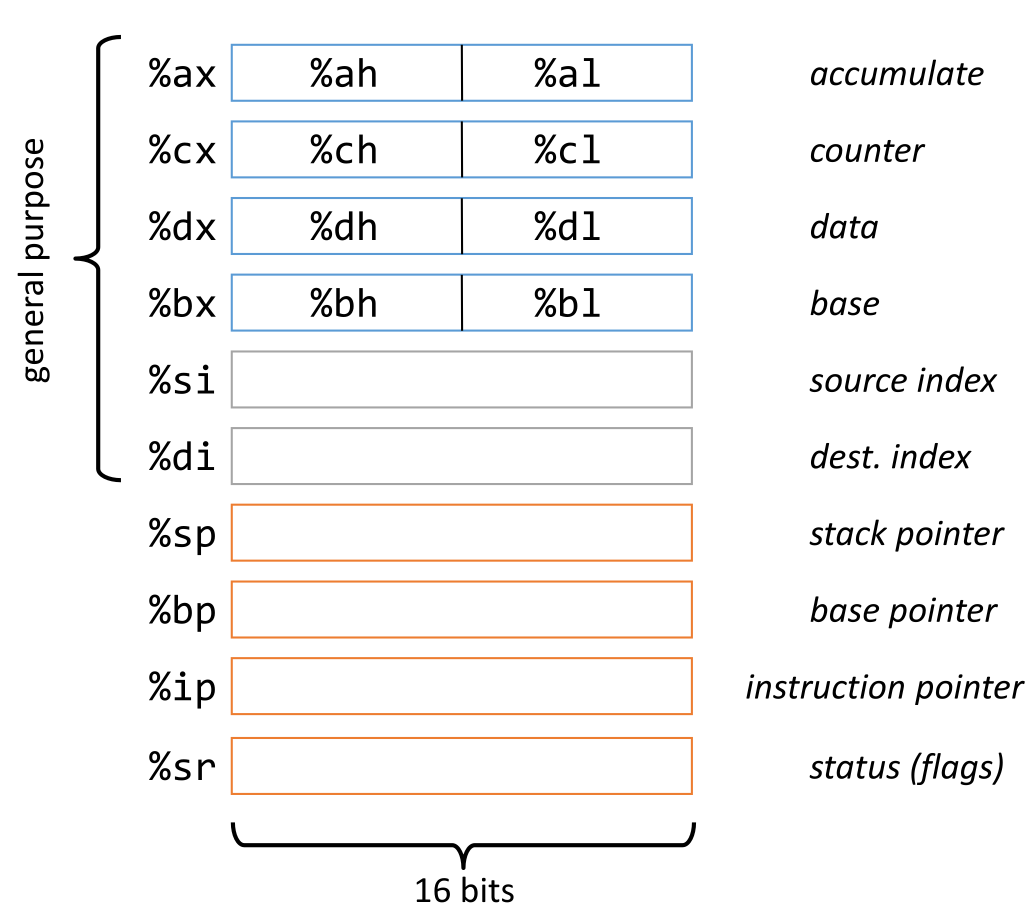
\includegraphics[width=0.8\textwidth]{09_8086.png}

\paragraph{80386 (ia32)}
This ISA is again an extension of the 8086. It extends all registers to $32$ bits, but still allows access to the lower $16$ bits and the high/low bits. The name for the full $32$ bit register are simple the original register names with an appended e.

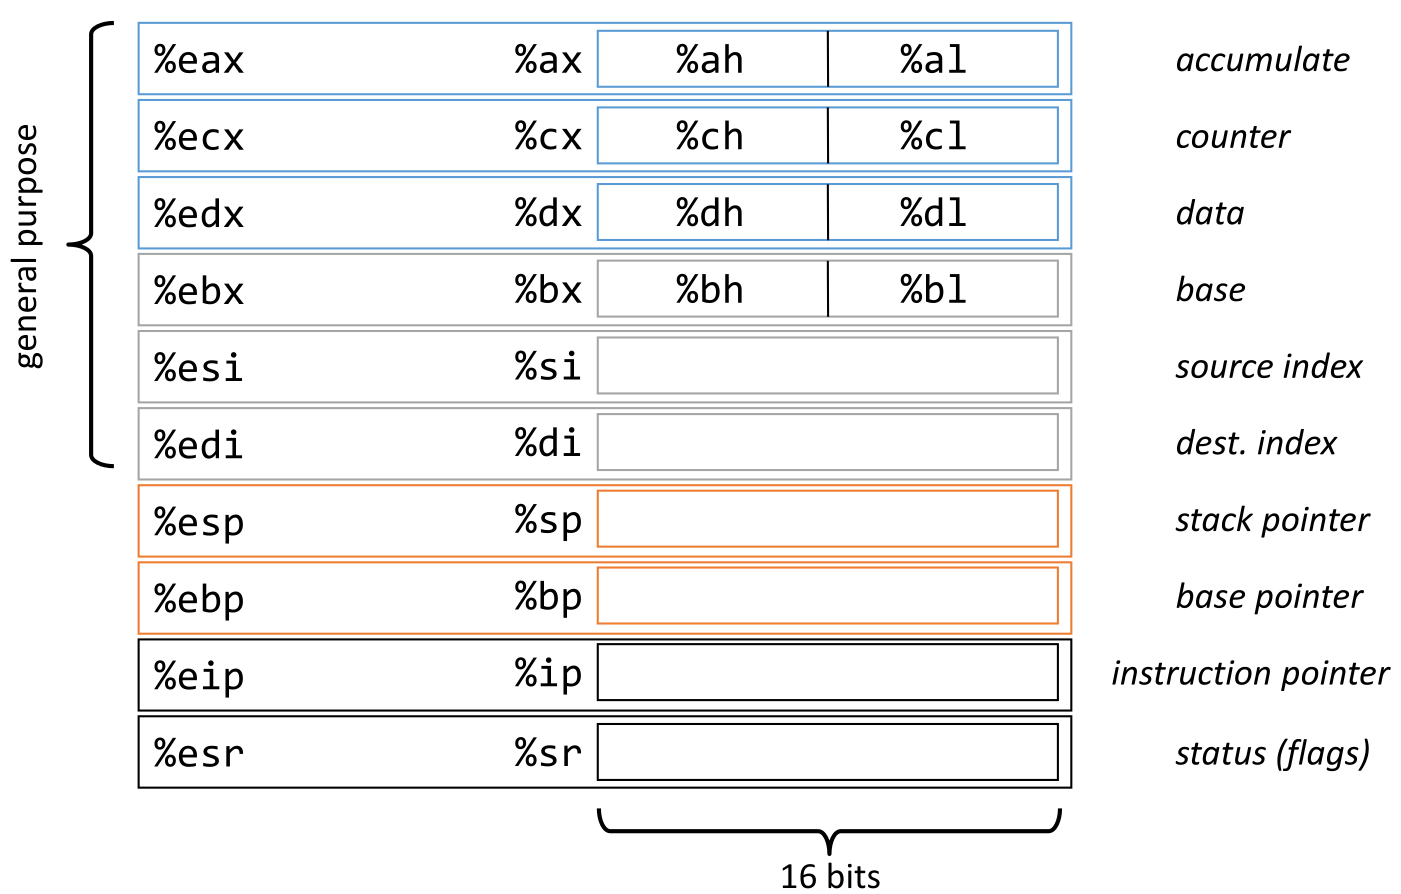
\includegraphics[width=0.8\textwidth]{09_80386.png}

\paragraph{x86-64}
In this ISA they have extended the $32$ bit registers to $64$ and doubled the number of general purpose registers compared to the ia32 (have a total of $16$). Again, they allow to access the lower $32$ (but not $16$) bits and the register name of ia32 was extended by prepending an r. Even though some registers still have some special name, we can actually use them for whatever we want.

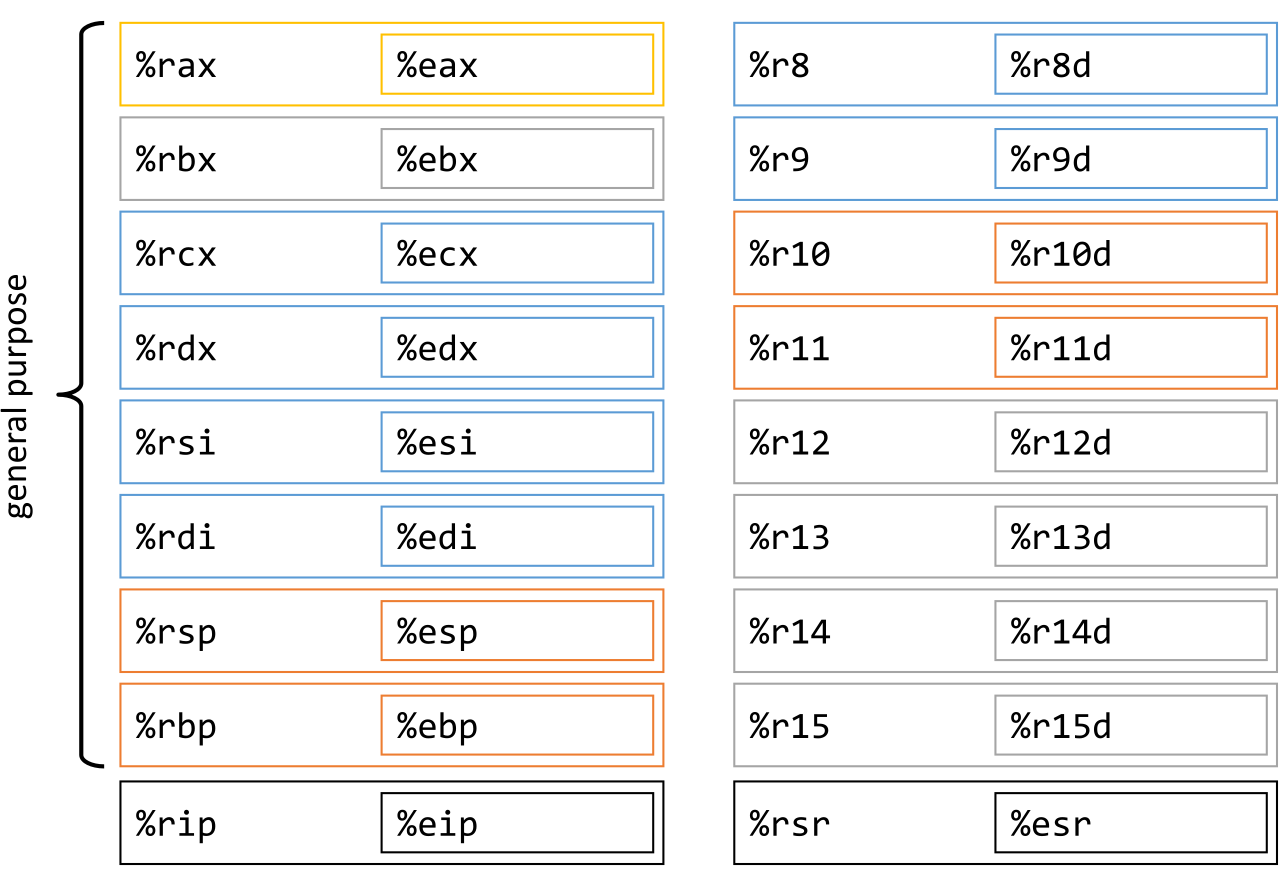
\includegraphics[width=0.8\textwidth]{09_x86-64.png}

\paragraph{Moving Data}
There are four flavours of the move instruction \code{movx Source, Dest}.
\begin{description}
    \item[movq:] move $8$-byte \textit{quad word}
    \item[movl:] move $4$-byte \textit{long word}
    \item[movw:] move $2$-byte \textit{word}
    \item[movb:] move $1$-byte \textit{byte}
\end{description}

There are three operand types.
\begin{description}
    \item[Immediate:] Constant integer in decimal or hexadecimal prepended by a $\$$ sign. The size can be $1$, $2$, $4$ or $8$ bytes.
    \item[Register:] Registers are referred by their name. There are general and special purpose registers.
    \item[Memory:] The general access mode is \code{D(Rb, Ri, S)} which is leads to a access of \code{Mem[Reg[Rb] + S * Reg[Ri] + D]}
        \begin{description}
            \item[D:] Constant displacement of size $1$, $2$ or $4$ bytes
            \item[Rb:] Base register; any of the 16 registers
            \item[Ri:] Index register; any of the registers except \code{\%rsp}
            \item[S:] Scale; any of $1$, $2$, $4$ or $8$. It is used for array access for arrays of certain type.
        \end{description}
\end{description}

Not all combinations of source and destination are available. So it is not possible to transfer data from memory to memory in one instruction.

\paragraph{Address Computation Instruction}
The command \code{lea Src, Dest} does not move any data, but rather calculates the address given by the address mode passed by \code{Src} and writes the address to \code{Dest}. This is useful when we need to compute an address without memory memory access, e.g. when creating a pointer. But it can also be used for general arithmetic.

The reason being is that the address calculation requires lot of hardware. Therefore, it does also make sense to use it for arithmetic.
